\documentclass[xcolor=svgnames]{beamer}

\mode<presentation>
{
  \usetheme{Warsaw}
  \setbeamertemplate{navigation symbols}{}
  \setbeamercovered{dynamic}
}

\usepackage[spanish,es-noshorthands]{babel}
\usepackage[utf8x]{inputenc}
\usepackage[T1]{fontenc}
\usepackage{csquotes}
\usepackage{tikz}
\usepackage{fancyvrb}
\usepackage[htt]{hyphenat}

\PrerenderUnicode{áéíóúÁÉÍÓÚçÇ}

\title[Introducción a Git]{Introducción al Sistema de Control de Versiones Distribuido Git}
\author{Antonio García Domínguez}
\date{\today}
\institute{Universidad de Cádiz \\\vspace{2em} 
\includegraphics{../../cc-by-sa}}

\AtBeginSection[]
{
  \begin{frame}<beamer>{Contenidos}
    \tableofcontents[currentsection,hideothersubsections]
  \end{frame}
}

\AtBeginSubsection[]
{
  \begin{frame}<beamer>{Contenidos}
    \tableofcontents[currentsection,subsectionstyle=show/shaded/hide]
  \end{frame}
}

\usetikzlibrary{calc,positioning,shapes,shapes.geometric}

% Semantic formatting
\newcommand*{\paquete}[1]{\texttt{#1}}
\newcommand*{\fichero}[1]{\textit{#1}}
\newcommand*{\rama}[1]{\structure{#1}}
\newcommand*{\tipo}[1]{\textit{#1}}
\newcommand*{\remoto}[1]{\structure{#1}}

% For formatting commands
\newcommand*{\inlinecmd}[1]{{\small\ttfamily\nohyphens{#1}}}
\newcommand*{\orden}[1]{{\scriptsize\ttfamily\$~\nohyphens{#1}\\}}

% For running Git commands and converting the ANSI escape sequences to LaTeX
\newcommand{\runcommand}[1]{\immediate\write18{#1}}
\newcommand{\showcommand}[2][cat]{%
  \runcommand{./err2out.sh '(#2)' | ansifilter -Lf | #1 | tee cmd.tmp}%
  {\scriptsize\ttfamily\input{cmd.tmp}}\runcommand{rm -f cmd.tmp}}
\newcommand{\runandshowcommand}[1]{
  \orden{#1}\showcommand{#1}}

% Required by ansifilter
\newcommand{\ws}[1]{\textcolor[rgb]{0,0,0}{#1}}

% For the diagrams talking about the existing types of VCS
\newenvironment{vcstypes}{
   \begin{tikzpicture}[
      node distance=6em,
      every path/.style={very thick},
      repo/.style={draw,rounded corners,fill=gray!50},
      wcopy/.style={draw,rounded corners,fill=green!20}]
}{\end{tikzpicture}}

\begin{document}

\begin{frame}
  \titlepage
\end{frame}

\begin{frame}{Contenidos}
  \tableofcontents[hideallsubsections]

  Materiales y transparencias para Linux en
  \url{http://osl2.uca.es/wikiformacion/index.php/Git} y
  \url{http://gitorious.org/curso-git-osluca}.
\end{frame}

\section{Introducción}

\subsection{Antecedentes}

\begin{frame}{Historia de los SCV}

  \begin{block}{Sin red, un desarrollador}
    \begin{description}
    \item[1972] Source Code Control System
    \item[1980] Revision Control System
    \end{description}
  \end{block}

  \begin{block}{Centralizados}
    \begin{description}
    \item[1986] Concurrent Version System
    \item[1999] Subversion (\enquote{CVS done right})
    \end{description}
  \end{block}

  \begin{block}{Distribuidos}
    \begin{description}
    \item[2001] Arch, monotone
    \item[2002] Darcs
    \item[2005] Git, Mercurial (hg), Bazaar (bzr)
    \end{description}
  \end{block}

\end{frame}

\begin{frame}{Historia de Git}

  \begin{block}{Antes de BitKeeper}
    Para desarrollar Linux, se usaban parches y \texttt{tar.gz}.
  \end{block}

  \begin{block}{BitKeeper}
    \begin{description}
    \item[02/2002] BitMover regala licencia BitKeeper (privativo)
    \item[04/2005] BitMover retira la licencia tras roces
    \end{description}
  \end{block}

  \begin{block}{Git}
    \begin{description}
    \item[04/2005] Linus Torvalds presenta Git, que ya reúne ramas
    \item[06/2005] Git se usa para gestionar Linux
    \item[02/2007] Git 1.5.0 es utilizable por mortales
    \item[09/2014] Última versión: Git 2.1.2
    \end{description}
  \end{block}

\end{frame}

\subsection{Tipos de SCV}

\begin{frame}{SCV centralizados}

  \begin{center}
    \begin{vcstypes}
      \draw[white] (3,2) rectangle (-3, -2);
      \node[repo]  (r)  {Repositorio central};

      \node<2->[wcopy,above right of=r] (w1) {Desarrollador A};
      \draw<2>[->,color=DarkGreen] (r) edge node[midway,right] {checkout} (w1);
      \draw<3>[<-,red] (r) edge node[midway,right] {commit} (w1);
      \draw<4->[-] (r) edge (w1);

      \node<2->[wcopy,below right of=r] (w2) {Desarrollador B};
      \draw<2>[->,color=DarkGreen] (r) edge node[midway,right] {checkout} (w2);
      \draw<3,5>[-] (r) edge (w2);
      \draw<4>[->,blue] (r) edge node[midway,right] {update} (w2);
    \end{vcstypes}
  \end{center}

  \begin{overprint}
    \onslide<1>
    \centering
    Tenemos nuestro repositorio central con todo dentro.

    \onslide<2>
    \centering
    Los desarrolladores crean \alert{copias de trabajo}.

    \onslide<3>
    \centering
    El desarrollador A manda sus cambios al servidor.

    \onslide<4>
    \centering
    El desarrollador B los recibe.

    \onslide<5>
    \centering ¿Y si se cae el servidor, o la red?
  \end{overprint}

\end{frame}

\begin{frame}{SCV distribuidos}

  \begin{center}
    \begin{vcstypes}
      \draw[white] (5,2) rectangle (-5, -2);

      \node[repo] (ra) at ( 0,-1) {Repositorio A};

      \node<2->[repo] (rb) at ( 3, 1) {Repositorio B};
      \draw<2>[->,color=DarkGreen] (ra) edge node[midway,right] {clone} (rb);
      \draw<3>[->,color=blue] (ra) edge node[midway,right] {pull} (rb);
      \draw<4>[<-,color=red] (ra) edge node[midway,right] {push} (rb);

      \node<5->[repo] (rc) at (-3, 1) {Repositorio C};
      \draw<5>[->,color=DarkGreen] (ra) edge node[midway,left] {clone} (rc);
      \draw<6>[<-,color=red] (ra) edge node[midway,left] {push} (rc);
      \draw<7>[<-,color=red] (ra) edge node[draw,fill=white,midway] {X} (rc);

      \draw<8>[->,color=red] (rc) edge node[midway,above] {push} (rb);

    \end{vcstypes}
  \end{center}

  \begin{overprint}
    \onslide<1> \centering Tenemos nuestro repositorio.

    \onslide<2> \centering Alguien \alert{clona} el repositorio.

    \onslide<3> \centering De vez en cuando se trae nuestros cambios recientes.

    \onslide<4> \centering De vez en cuando nos manda sus cambios.

    \onslide<5> \centering Viene otro desarrollador.

    \onslide<6> \centering Intenta hacer sus cambios locales...

    \onslide<7> \centering Pero no le funciona, o no tiene permisos para ello.

    \onslide<8> \centering Se los pasa al otro desarrollador sin más.

    \onslide<9> \centering La diferencia entre los repositorios es
    \emph{social}, no técnica.
  \end{overprint}

\end{frame}

\begin{frame}{Ventajas de un SCV distribuido (I)}

  \begin{block}{Rapidez}
    \begin{itemize}
    \item Todo se hace en local: el disco duro es más rápido que la
      red, y cuando esté todo en caché será más rápido aún
    \item Clonar un repositorio Git suele tardar \emph{menos} que
      crear una copia de trabajo de SVN, y ocupa menos
    \end{itemize}
  \end{block}

  \pause

  \begin{block}{Revisiones pequeñas y sin molestar}
    \begin{itemize}
    \item Nadie ve nada nuestro hasta que lo mandamos
    \item Podemos ir haciendo revisiones pequeñas intermedias
    \item Sólo mandamos cuando compila y supera las pruebas
    \item Podemos hacer experimentos de usar y tirar
    \end{itemize}
  \end{block}

\end{frame}

\begin{frame}{Ventajas de un SCV distribuido (II)}
  \begin{block}{Trabajo sin conexión}
    \begin{itemize}
    \item En el tren, avión, autobús, etc.
    \item Aunque no tengamos permisos de escritura
    \item Aunque se caiga la red, se puede colaborar
    \end{itemize}
  \end{block}

  \pause

  \begin{block}{Robustez}
    Falla el disco duro del repositorio bendito. ¿Qué hacer?
    \begin{itemize}
    \item Centralizado: copias de seguridad
    \item Distribuido: copias de seguridad y/o colaborar por otros medios
    \end{itemize}
  \end{block}
\end{frame}

\begin{frame}{Cuándo NO usar Git}

  \begin{block}{Git no escala ante muchos ficheros binarios}
    \begin{itemize}
    \item No sirve para llevar las fotos
    \item Ni para almacenar vídeos
    \end{itemize}
  \end{block}

  \begin{block}{Git no guarda metadatos}
    No sirve como sistema de copias de seguridad
  \end{block}

\end{frame}

\section[Local]{Trabajo local}

\subsection{Preparación}

\begin{frame}{Instalación de Git (Windows)}
  \begin{block}{Clientes libres}
    \begin{itemize}
    \item El original: \structure{Git for Windows} (\url{http://msysgit.github.io/})
      \begin{itemize}
      \item ``Git Bash'' permite usar todas las órdenes típicas en Linux
      \item ``Git GUI'' permite preparar y hacer revisiones de forma gráfica
      \end{itemize}
    \item Como TortoiseSVN: \structure{TortoiseGit} (\url{http://code.google.com/p/tortoisegit/})
      \begin{itemize}
      \item Para aprovechar toda la potencia de Git, hay que complementarlo con los de arriba
      \end{itemize}
    \end{itemize}
  \end{block}

  \begin{block}{Clientes privativos}
    \begin{itemize}
    \item \$79/persona: \structure{SmartGit} (\url{http://www.syntevo.com/smartgit/})
    \item Gratis por ahora: \structure{SourceTree} (\url{http://www.sourcetreeapp.com/})
    \end{itemize}
  \end{block}
\end{frame}

\begin{frame}{Instalación de Git (Linux)}
  \begin{block}{Ubuntu Linux 14.04}
    \begin{itemize}
    \item \paquete{git} trae todo lo fundamental
    \item \paquete{git-all} aporta muchos extras
    \item \paquete{tkdiff} para resolver conflictos
    \end{itemize}
  \end{block}

  \begin{block}{SuSE}
    Hay paquetes actualizados en el openSUSE Build Service
    (\paquete{devel:tools:scm} $\rightarrow$ \paquete{git}).
  \end{block}
\end{frame}

\begin{frame}{Configuración inicial (Windows): acceso a opciones}
  \begin{center}
    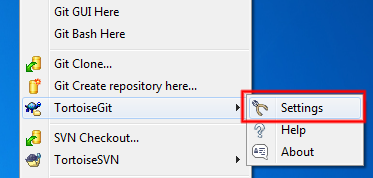
\includegraphics[width=\textwidth,height=.8\textheight,keepaspectratio]{tomas/configinicial-00-menu}
  \end{center}
\end{frame}

\begin{frame}{Configuración inicial (Windows): datos personales}
  \begin{center}
    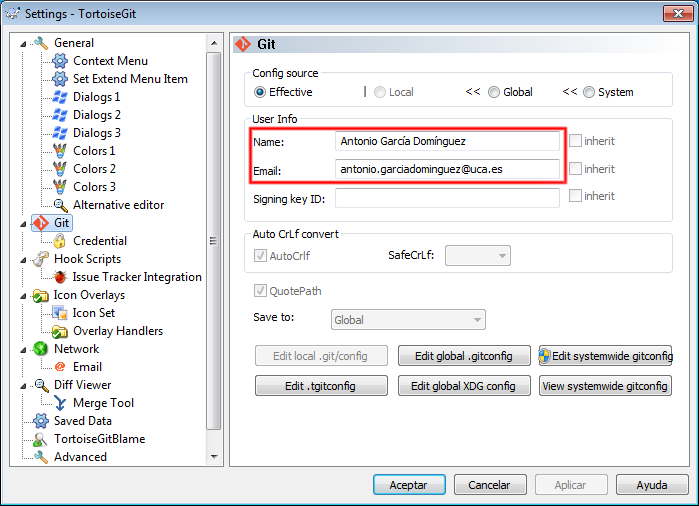
\includegraphics[width=\textwidth,height=.8\textheight,keepaspectratio]{tomas/configinicial-01-pantalla}
  \end{center}
\end{frame}

\begin{frame}{Configuración inicial (Windows): gestor de credenciales}
  \begin{center}
    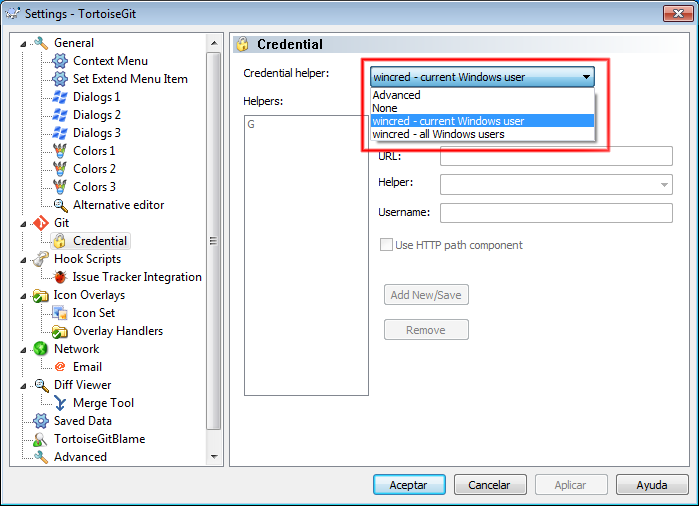
\includegraphics[width=\textwidth,height=.8\textheight,keepaspectratio]{tomas/configinicial-02-creds}
  \end{center}
\end{frame}

\begin{frame}{Configuración inicial (Linux)}
  \framesubtitle{Cambiamos la configuración global en \fichero{\$HOME/.gitconfig}}

  \begin{block}{Identificación}
    \orden{git config {-}-global user.name "Mi Nombre"}
    \orden{git config {-}-global user.email mi@correo}
  \end{block}

  \begin{block}{Editor: por defecto Vi/Vim}
    \orden{git config {-}-global core.editor emacs}
  \end{block}

  \begin{block}{Herramienta para resolver conflictos}
    \orden{git config {-}-global merge.tool tkdiff}
  \end{block}

  \begin{block}{Algunos alias útiles}
    \orden{git config {-}-global alias.ci commit}
    \orden{git config {-}-global alias.st status}
    \orden{git config {-}-global alias.ai "add -i"}
  \end{block}

\end{frame}

% Limpiamos el área de trabajo
\runcommand{rm -rf ejemplo}

\begin{frame}{Creación de un repositorio (Windows): orden inicial}
  Sólo tenemos que crear un nuevo directorio y decirle a Git que cree
  un repositorio ahí.

  \begin{center}
    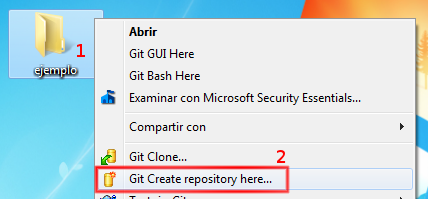
\includegraphics[width=\textwidth,height=.5\textheight,keepaspectratio]{tomas/crearrepo-00-menu}
  \end{center}
\end{frame}

\begin{frame}{Creación de un repositorio (Windows): repositorios ``pelados''}
  Un repositorio \emph{bare} no tiene un directorio de trabajo
  asociado: sólo lleva el histórico. Normalmente se usan en
  servidores, como en \url{des-sinf.uca.es}.

  Ahora queremos uno normal, por lo que dejamos la caja sin marcar.

  \begin{center}
    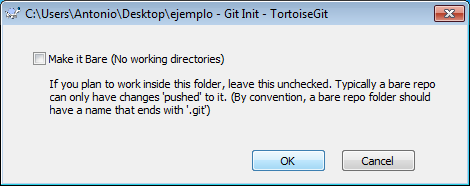
\includegraphics[width=\textwidth,height=.5\textheight,keepaspectratio]{tomas/crearrepo-01-bare}
  \end{center}
\end{frame}

\begin{frame}{Creación de un repositorio (Linux)}
  \runandshowcommand{mkdir ejemplo}
  \orden{cd ejemplo}
  \orden{git init}
  \showcommand{cd ejemplo; git init | fold -sw 70; git config user.name Antonio; git config user.email a@b.com; git config color.ui always; git config rerere.enabled false}
\end{frame}

\begin{frame}[t]{Nuestra primera revisión en la rama master (Windows)}

  \begin{overprint}
    \onslide<1>
    \begin{center}
      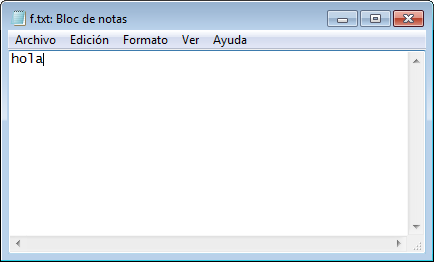
\includegraphics[width=\textwidth,height=.6\textheight,keepaspectratio]{tomas/primercommit-06-newfile}

      \vfill

      Creamos un fichero \fichero{f.txt} con ``hola''.
    \end{center}

    \onslide<2>
    \begin{center}
      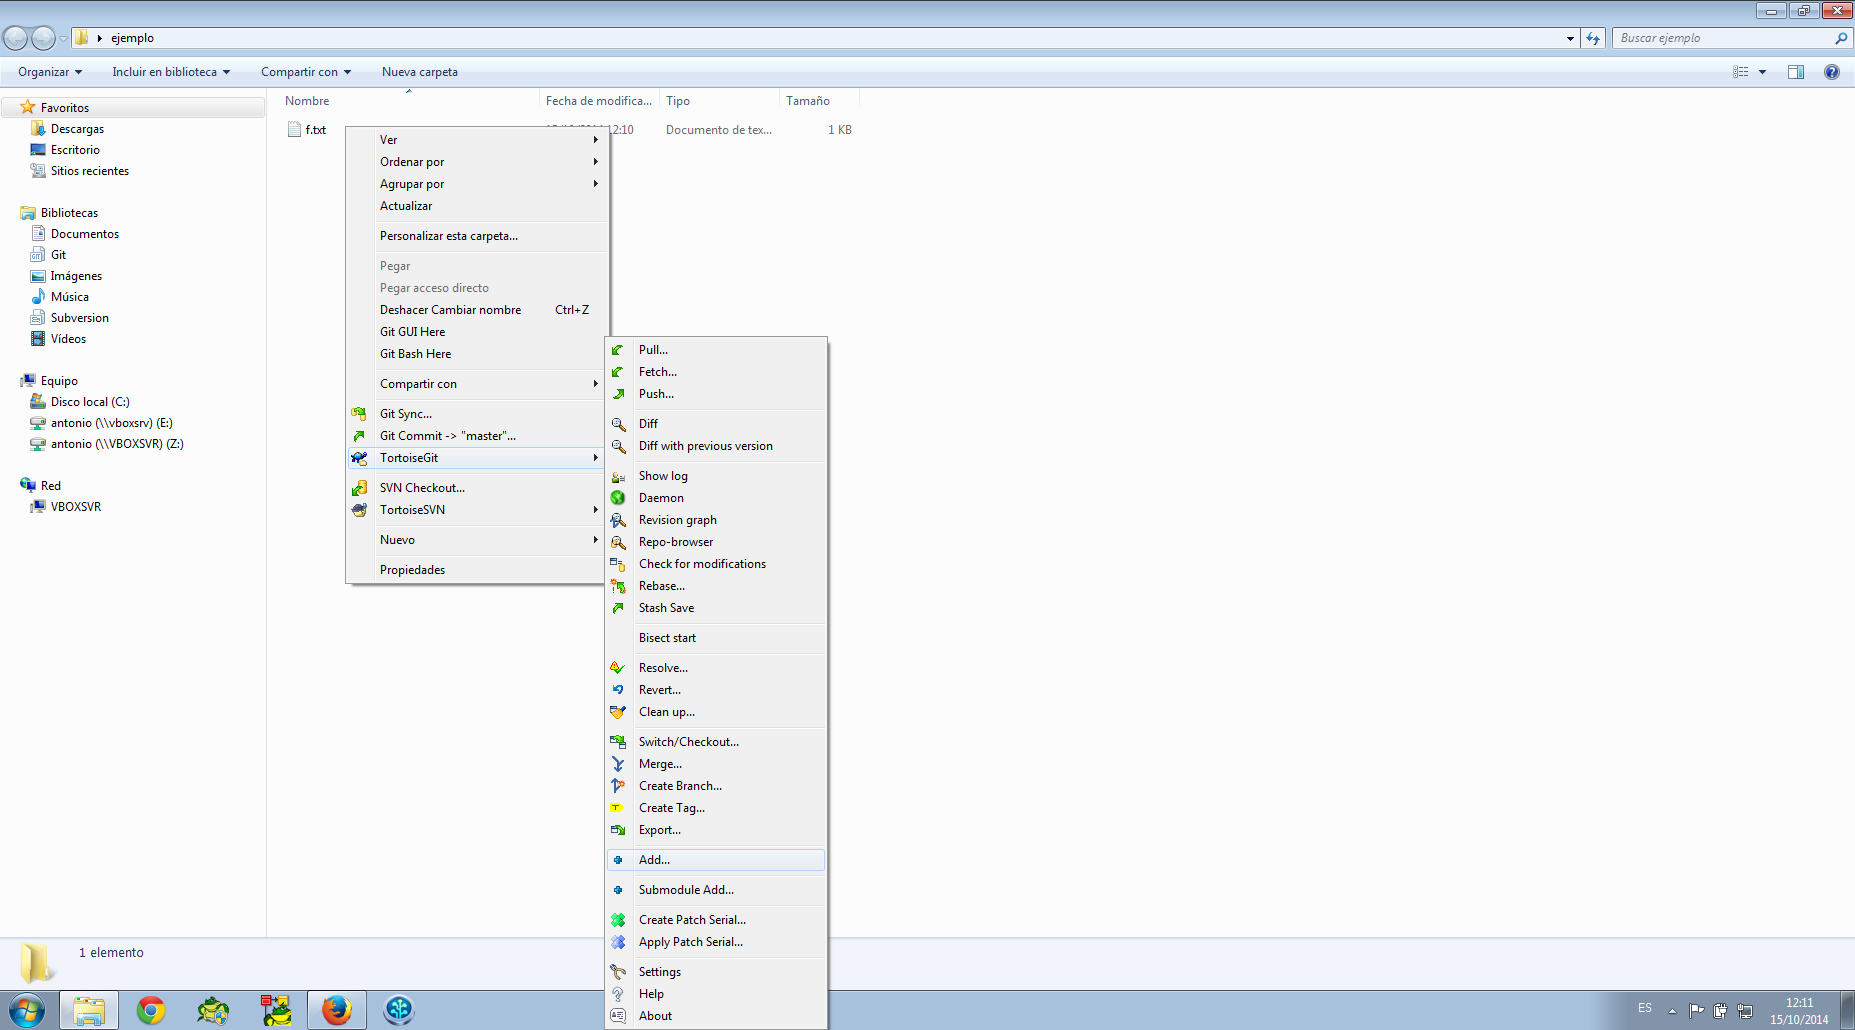
\includegraphics[width=\textwidth,height=.6\textheight,keepaspectratio]{tomas/primercommit-00-add}

      \vfill

      Añadimos el fichero a control de versiones mediante ``Add''.
    \end{center}

    \onslide<3>
    \begin{center}
      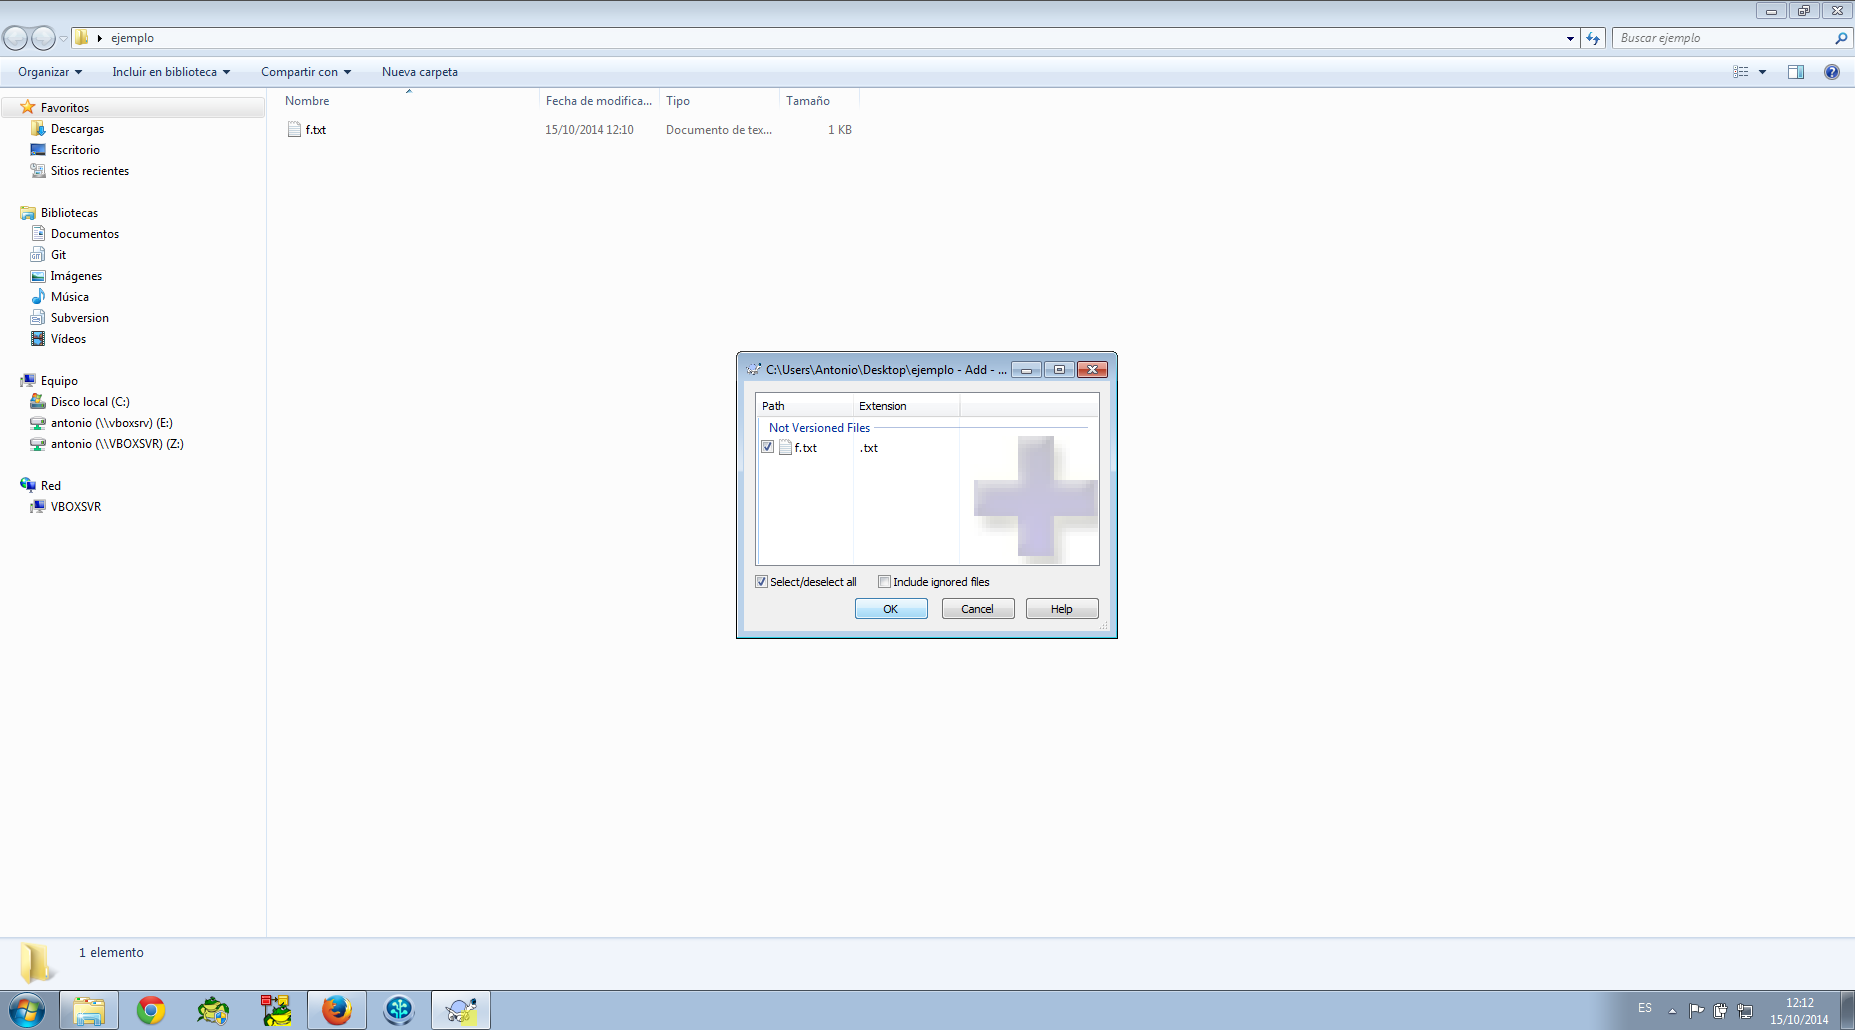
\includegraphics[width=\textwidth,height=.6\textheight,keepaspectratio]{tomas/primercommit-01-dlgadd}

      \vfill

      Marcamos el fichero y pulsamos en ``OK''.
    \end{center}

    \onslide<4>
    \begin{center}
      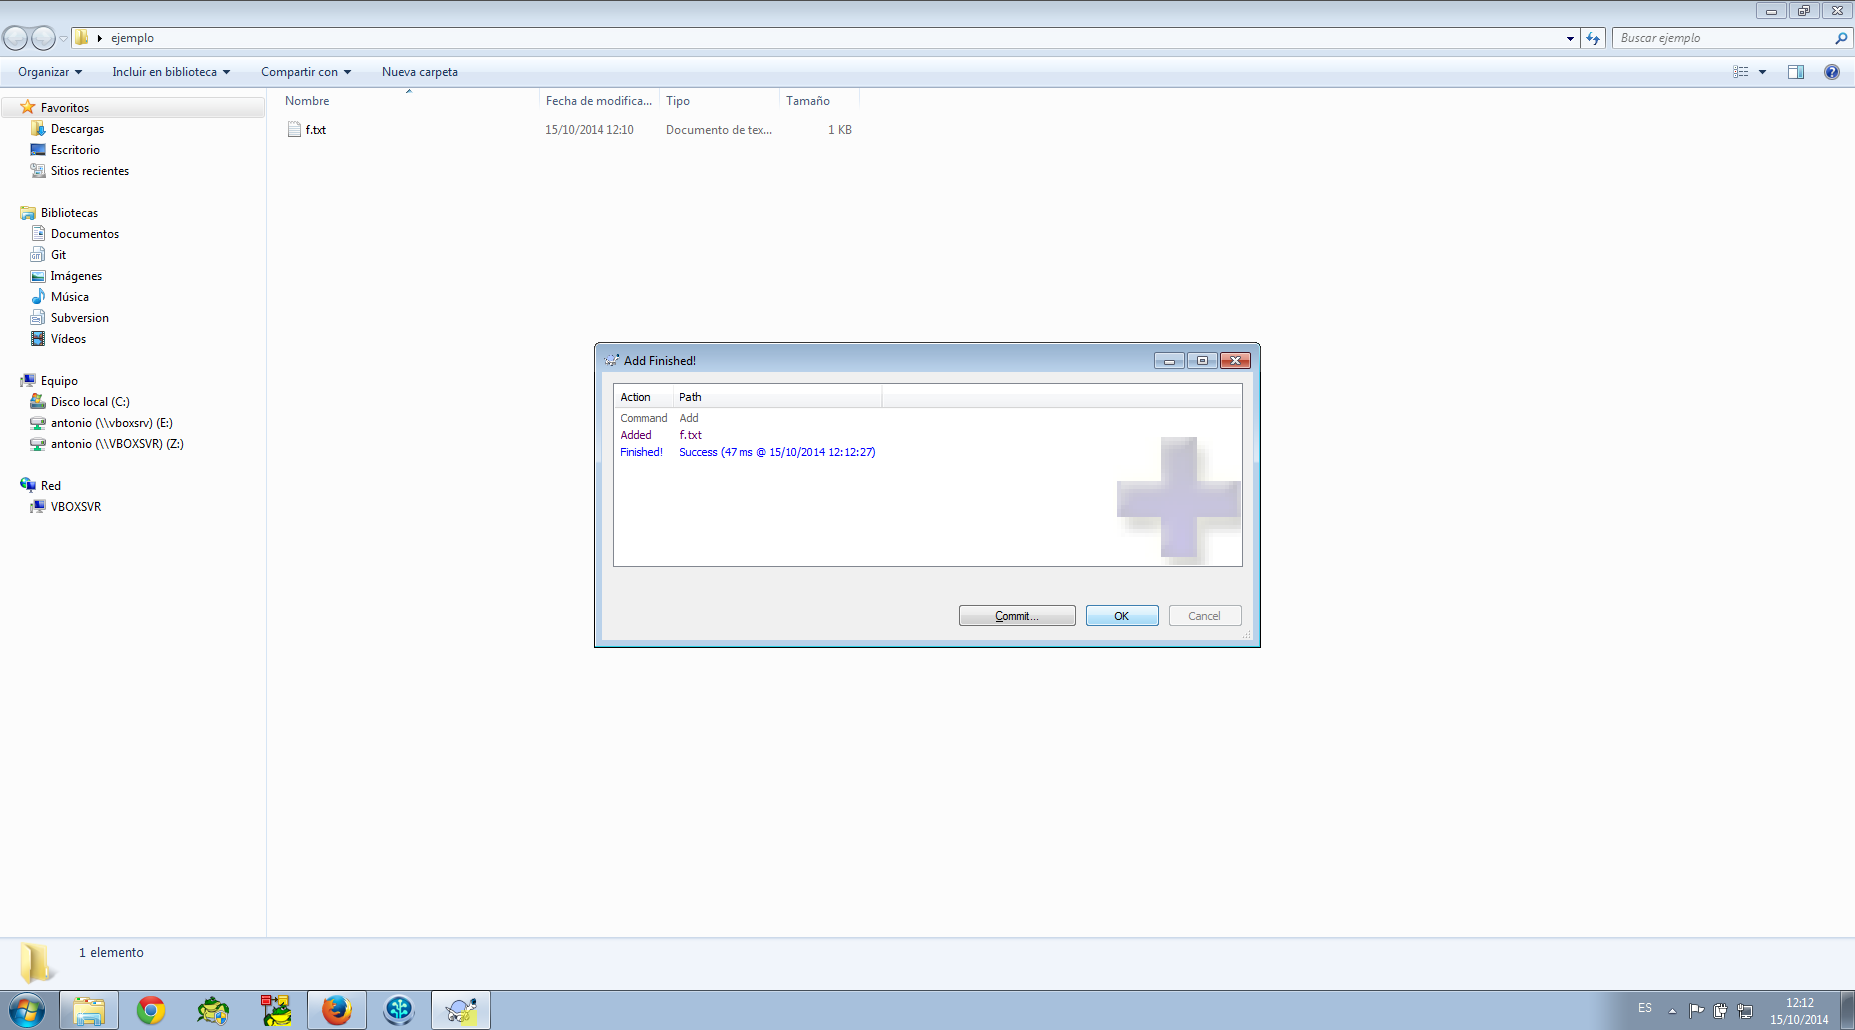
\includegraphics[width=\textwidth,height=.6\textheight,keepaspectratio]{tomas/primercommit-02-success}

      \vfill

      Se nos confirma el añadido.
    \end{center}

    \onslide<5>
    \begin{center}
      \vspace{.15\textheight}

      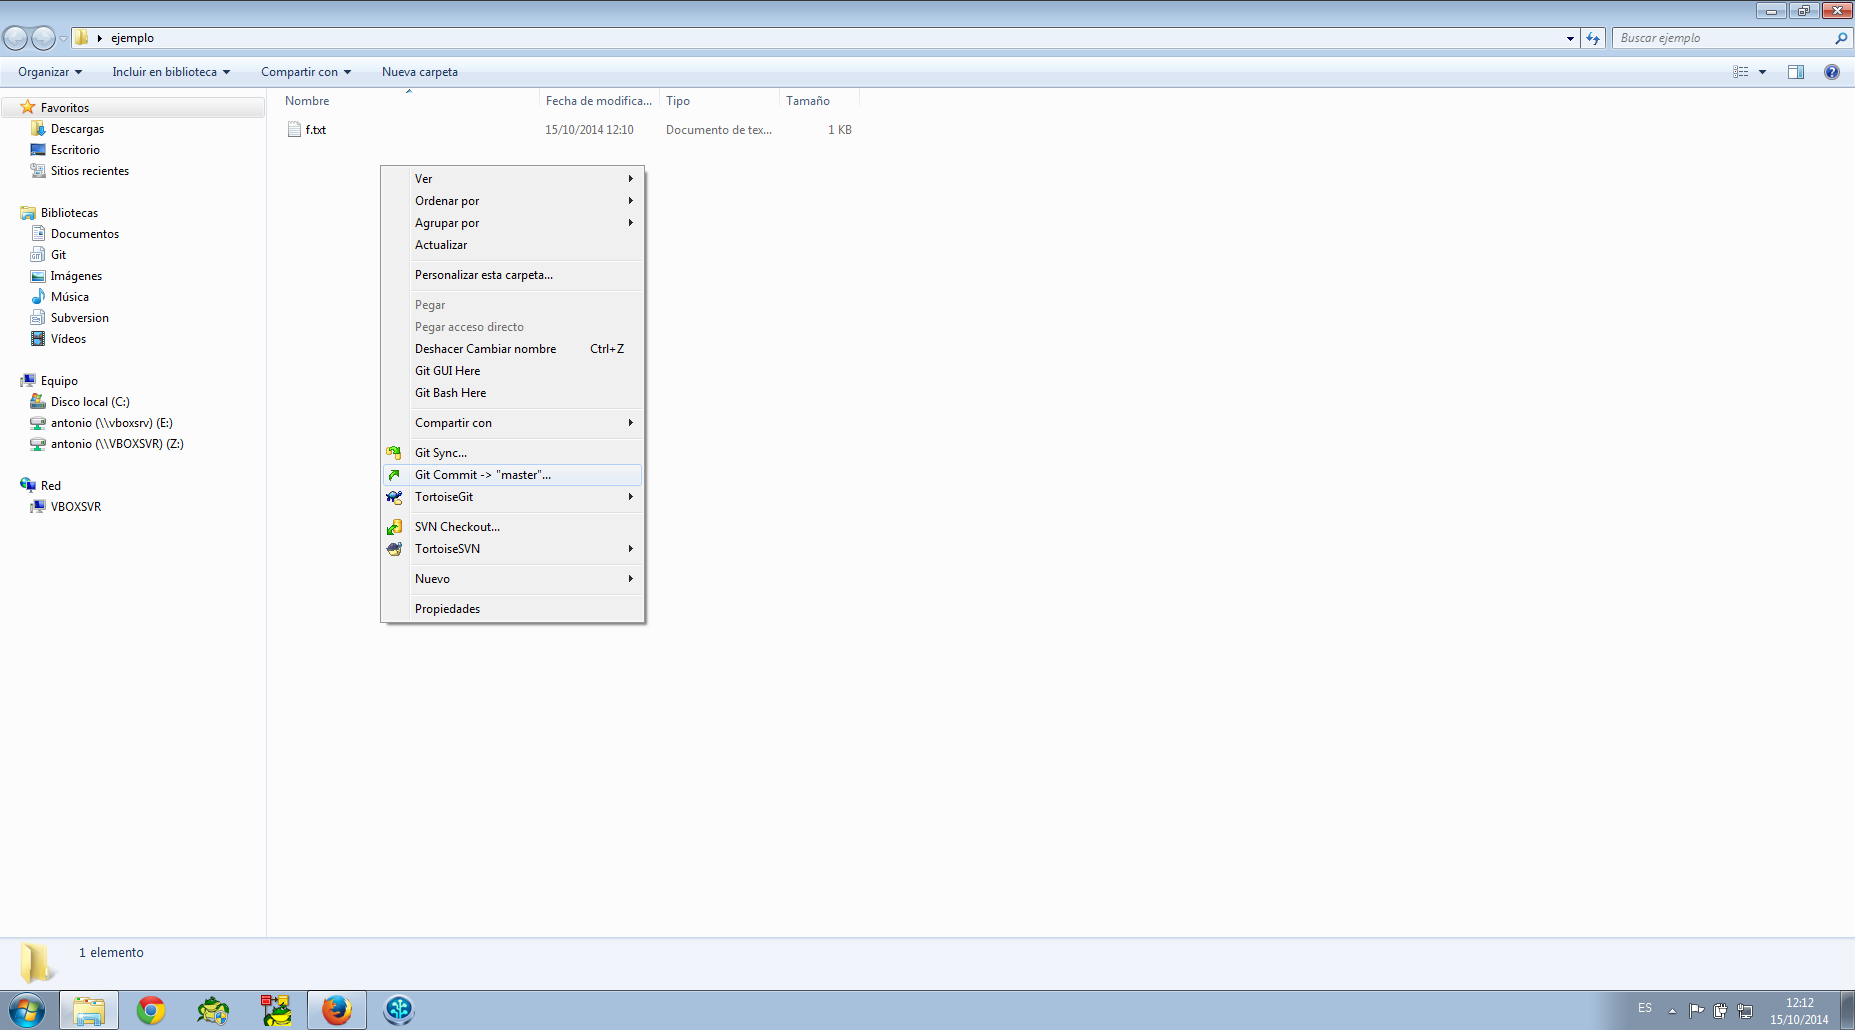
\includegraphics[width=\textwidth,height=.6\textheight,keepaspectratio]{tomas/primercommit-03-commit}

      \vspace{.15\textheight}

      Usamos ``Commit'' para iniciar la creación de la revisión.
    \end{center}

    \onslide<6>
    \begin{center}
      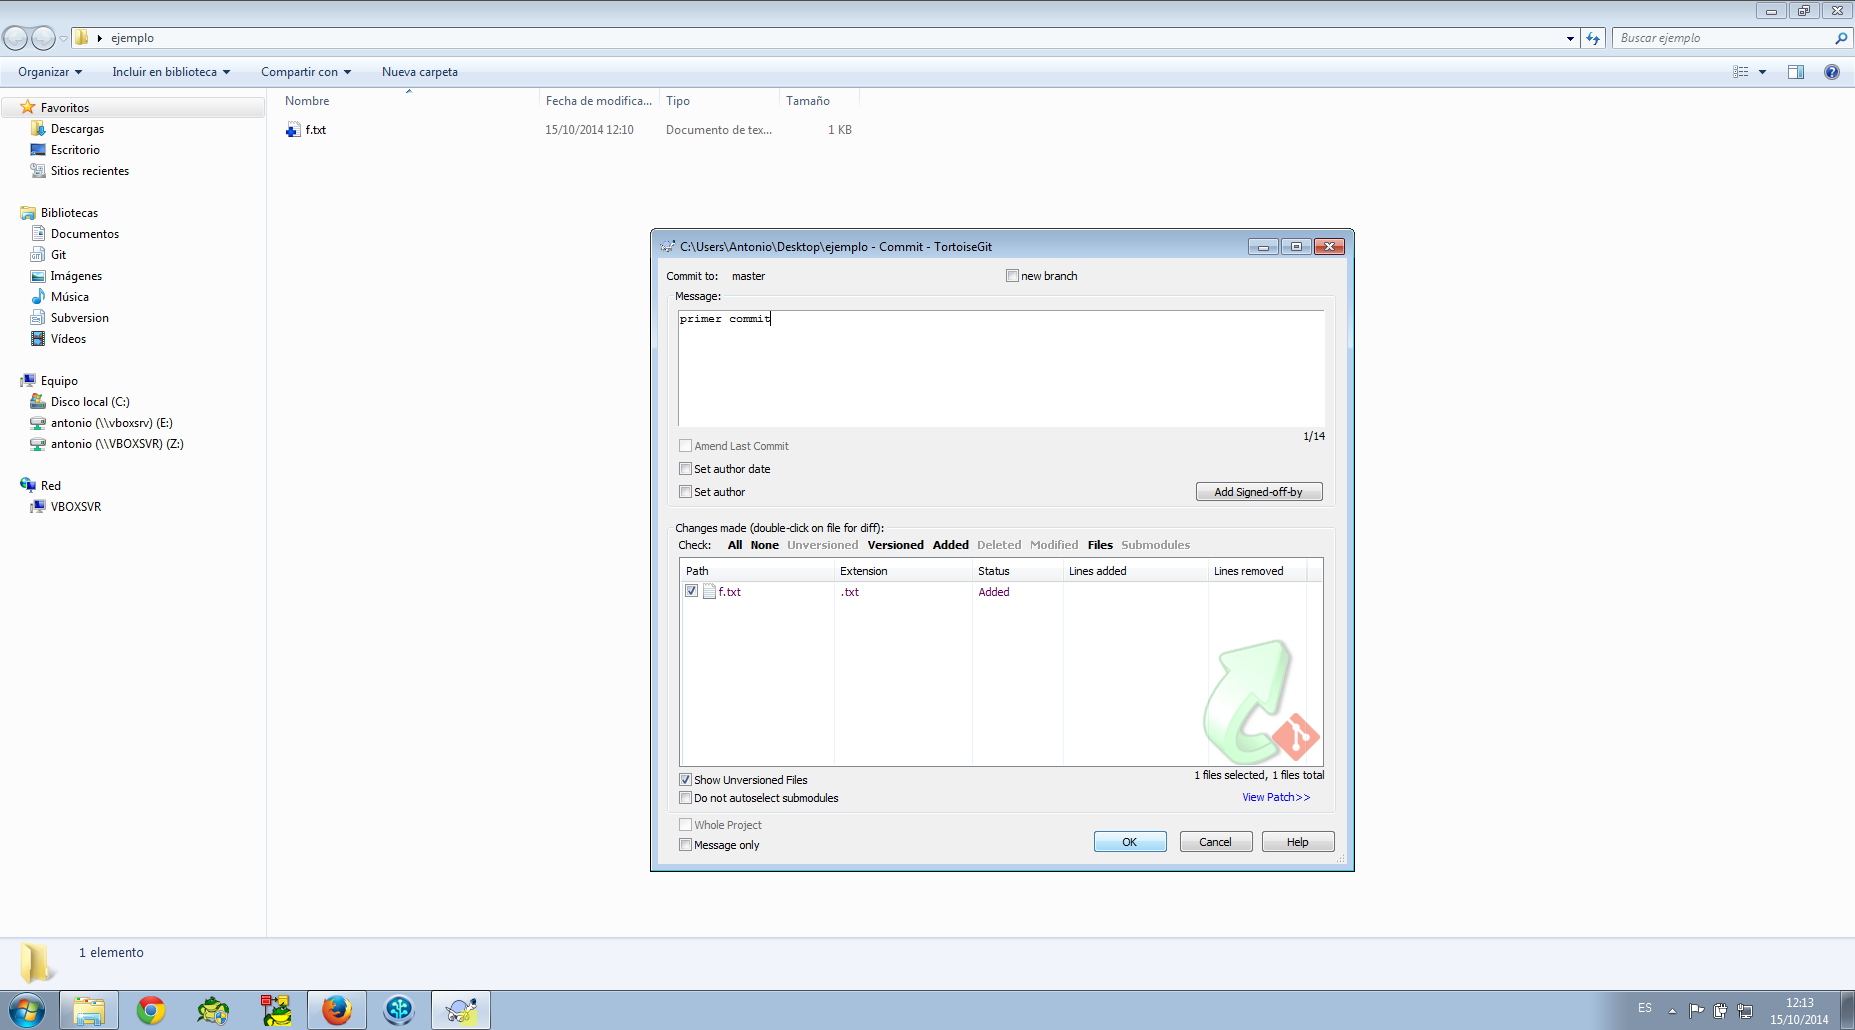
\includegraphics[width=\textwidth,height=.6\textheight,keepaspectratio]{tomas/primercommit-04-dlgcommit}

      \vfill

      Introducimos el mensaje. En \url{des-sinf.uca.es}, no debemos olvidar poner \texttt{refs \#{}XYZ} al final de la primera línea.
    \end{center}

    \onslide<7-8>
    \begin{center}
      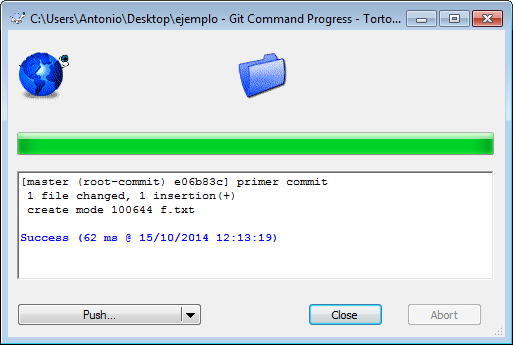
\includegraphics[width=\textwidth,height=.6\textheight,keepaspectratio]{tomas/primercommit-05-okcommit}

      \vfill

      Se nos confirma el commit. \alert{Ojo}: no se envía a ningún lado. Para eso existe ``Push'', que veremos después.
    \end{center}
  \end{overprint}

\end{frame}

\begin{frame}{Nuestra segunda revisión en la rama master (Windows)}

  \begin{overprint}
    \onslide<1>
    \begin{center}
      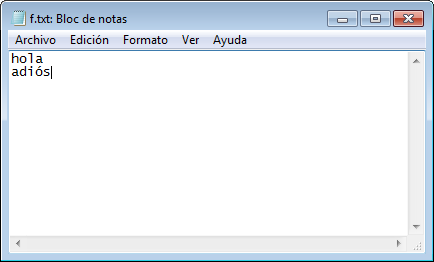
\includegraphics[width=\textwidth,height=.6\textheight,keepaspectratio]{tomas/segundocommit-00-changedfile}

      Añadimos una línea con ``adiós'' a \fichero{f.txt}.
    \end{center}

    \onslide<2>
    \begin{center}
      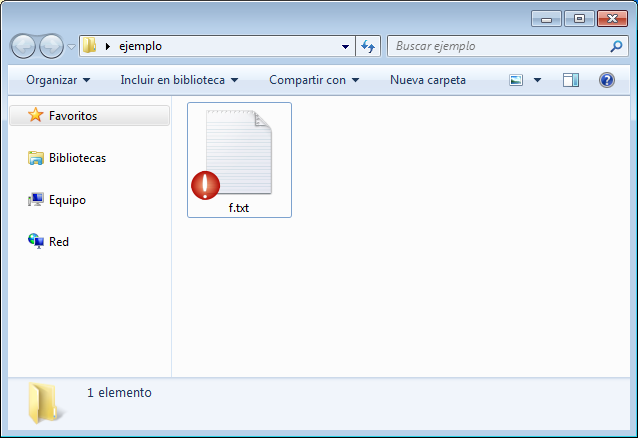
\includegraphics[width=\textwidth,height=.6\textheight,keepaspectratio]{tomas/segundocommit-01-emblem}

      Se cambia el emblema de \fichero{f.txt}, indicando que su contenido no coincide con el de la revisión actual.
    \end{center}

    \onslide<3>
    \begin{center}
      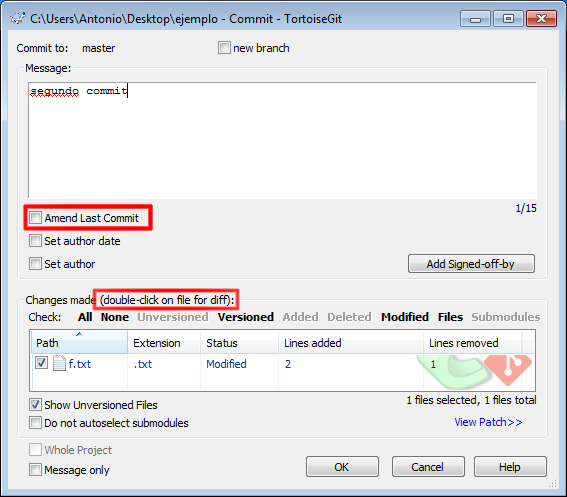
\includegraphics[width=\textwidth,height=.6\textheight,keepaspectratio]{tomas/segundocommit-02-dlgcommit}

      Creamos la segunda revisión con el mensaje ``segundo
      commit''. Podemos arreglar la última revisión (siempre que no la
      hayamos subido) o ver qué cambios hemos introducido.
    \end{center}

    \onslide<4>
    \begin{center}
      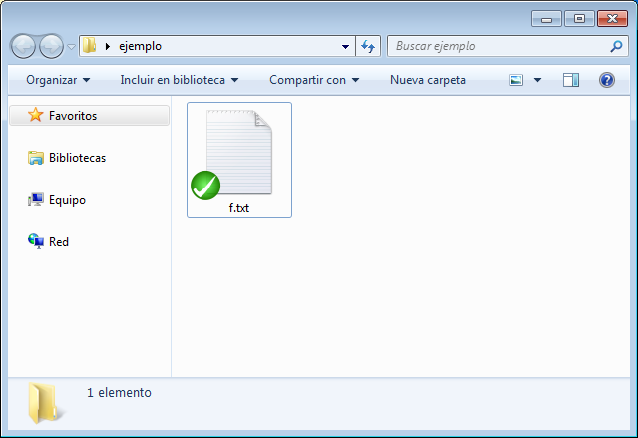
\includegraphics[width=\textwidth,height=.6\textheight,keepaspectratio]{tomas/segundocommit-03-emblemok}

      Se cambia el emblema de \fichero{f.txt}, indicando que su contenido sí coincide con el de la revisión actual.
    \end{center}
  \end{overprint}
\end{frame}

\begin{frame}{Nuestras dos primeras revisiones en la rama master (Linux)}
  \orden{echo "hola" > f.txt}
  \runcommand{echo "hola" | tee ejemplo/f.txt}
  \orden{git add f.txt}
  \showcommand{cd ejemplo; git add f.txt}
  \orden{git commit -m "primer commit"}
  \showcommand{cd ejemplo; git commit -m "primer commit"}
  \orden{echo "adios" {>}> f.txt}
  \runcommand{echo "adios" | tee -a ejemplo/f.txt}
  \orden{git add f.txt}
  \showcommand{cd ejemplo; git add f.txt}
  \orden{git commit -m "segundo commit"}
  \showcommand{cd ejemplo; git commit -m "segundo commit"}
\end{frame}

\begin{frame}{Preguntas tras estas dos revisiones}
  \begin{itemize}
  \item ¿Qué es ese identificador después de \enquote{root-commit}?
  \item ¿Dónde se guardan mis cosas?
  \item ¿\enquote{\texttt{git add}} dos veces en Linux?
  \end{itemize}
\end{frame}

\subsection{Conceptos}

%% MODELO DE DATOS

\begin{frame}{Modelo de datos de Git}
  \begin{block}{Características}
    \begin{itemize}
    \item Un repositorio es un grafo orientado acíclico de objetos
    \item Hay 4 tipos de objetos: \tipo{commit}, \tipo{tree},
      \tipo{blob} y \tipo{tag}
    \item Los objetos son direccionables por contenido (resumen SHA1)
    \end{itemize}
  \end{block}

  \begin{block}{Consecuencias del diseño}
    \begin{itemize}
    \item Los objetos son inmutables: al cambiar su contenido, cambia
      su SHA1
    \item Git \emph{no} gestiona información de ficheros movidos y demás
    \item Git \emph{nunca} guarda más de un objeto una vez en el DAG,
      aunque aparezca en muchos sitios
    \end{itemize}
  \end{block}
\end{frame}

\begin{frame}{Modelo de datos de Git: revisiones (\tipo{commits})}
  \begin{block}{Contenido}
    \begin{itemize}
    \item Fecha, hora, autoría, fuente y un mensaje
    \item Referencia a revisión padre y a un \tipo{tree}
    \end{itemize}
  \end{block}

  \vfill

  \orden{git cat-file -p HEAD}
  \showcommand{cd ejemplo; git cat-file -p HEAD}
\end{frame}

\begin{frame}{Modelo de datos de Git: árboles (\tipo{trees})}
  \begin{block}{Contenido}
    \begin{itemize}
    \item Lista de \tipo{blobs} y \tipo{trees}
    \item Separa el nombre de un fichero/directorio de su contenido
    \item Sólo gestiona los bits de ejecución de los ficheros
    \item No se guardan directorios vacíos
    \end{itemize}
  \end{block}

  \vfill

  \orden{git cat-file -p HEAD:}
  \showcommand{cd ejemplo; git cat-file -p HEAD:}
\end{frame}

\begin{frame}{Modelo de datos de Git: ficheros (\tipo{blobs})}
  \begin{block}{Contenido}
    Secuencias de bytes sin ningún significado particular.
  \end{block}

  \vfill

  \orden{git cat-file -p HEAD:f.txt}
  \showcommand{cd ejemplo; git cat-file -p HEAD:f.txt}
\end{frame}

\begin{frame}{Modelo de datos de Git: etiquetas (\tipo{tags})}
  \begin{block}{Contenido}
    \begin{itemize}
    \item Referencias simbólicas inmutables a otros objetos
    \item Normalmente apuntan a \tipo{commits}
    \item Pueden firmarse mediante GnuPG, protegiendo la integridad de
      todo el historial hasta entonces
    \end{itemize}
  \end{block}

  \vfill

  \orden{git tag -a v1.0 -m "version 1.0" HEAD}
  \runcommand{cd ejemplo; git tag -a v1.0 -m "version 1.0" HEAD}
  \orden{git cat-file -p v1.0}
  \showcommand{cd ejemplo; git cat-file -p v1.0}
\end{frame}

%%% MODELO DE DATOS

\begin{frame}{Estructura física de un repositorio Git}
  \begin{block}{Partes de un repositorio Git}
    \begin{itemize}
    \item Directorio de trabajo
    \item Grafo de objetos: directorio oculto \fichero{.git} en repositorios normales
    \item Área de preparación: \fichero{.git/index}
    \end{itemize}
  \end{block}

  \vfill

  \orden{ls .git}
  \showcommand{cd ejemplo; ls -C --color=always .git}
\end{frame}

\begin{frame}[t]{Algunos de los ficheros en \fichero{.git}}

  \begin{overlayarea}{\textwidth}{2cm}
    \only<1>{
      \begin{block}{config}
        Contiene la configuración local.
      \end{block}
    }
    \only<2>{
      \begin{block}{HEAD}
        Referencia simbólica a la revisión sobre la que estamos
        trabajando.
      \end{block}
    }
    \only<3>{
      \begin{block}{hooks}
        Manejadores de eventos. Ahora sólo tenemos ejemplos.
      \end{block}
    }
    \only<4>{
      \begin{block}{index}
        Contiene el área de preparación (la veremos después).
      \end{block}
    }
    \only<5>{
      \begin{block}{info/exclude (también .gitignore y/o global)}
        Patrones de ficheros a ignorar.
      \end{block}
    }
    \only<6>{
      \begin{block}{logs}
        Historial de las referencias: medida de seguridad.
      \end{block}
    }
    \only<7>{
      \begin{block}{refs}
        Referencias simbólicas a puntas de cada rama y etiquetas.
      \end{block}
    }
    \only<8>{
      \begin{block}{objects}
        Objetos, sueltos (gzip) o empaquetados (delta + gzip).
      \end{block}
    }
  \end{overlayarea}

  \begin{overlayarea}{\textwidth}{6cm}
    \only<1>{
      \orden{cat config}
      \showcommand{cat ejemplo/.git/config | sed -n '1,/logallrefupdates/p'}
    }
    \only<2>{
      \orden{cat description}
      \showcommand{cat ejemplo/.git/description}
    }
    \only<3>{
      \orden{cat HEAD}
      \showcommand{cat ejemplo/.git/HEAD}
    }
    \only<4>{
      \orden{ls hooks | head -5}
      \showcommand{ls --color=always ejemplo/.git/hooks | head -5}
    }
    \only<5>{
      \orden{git ls-files -s}
      \showcommand{cd ejemplo; git ls-files -s}
    }
    \only<6>{
      \orden{cat info/exclude}
      \showcommand{cat ejemplo/.git/info/exclude}
    }
    \only<7>{
      \orden{git reflog}
      \showcommand{cd ejemplo; git reflog}
    }
    \only<8>{
      \orden{ls -R refs}
      \showcommand{ls -CR --color=always ejemplo/.git/refs}
    }
    \only<9>{
      \orden{ls objects}
      \showcommand{ls -C --color=always ejemplo/.git/objects | ./chomp-last-newline.pl}
      \orden{ls objects/pack}
      \runcommand{ls -C ejemplo/.git/objects/pack}
      \orden{git gc}
      \runcommand{cd ejemplo; git gc}
      \orden{ls objects}
      \showcommand{ls -C --color=always ejemplo/.git/objects | ./chomp-last-newline.pl}
      \orden{ls objects/pack}
      \showcommand{ls -C --color=always ejemplo/.git/objects/pack | ./chomp-last-newline.pl}
    }
  \end{overlayarea}

\end{frame}

\begin{frame}{Área de preparación, caché o índice}
  \begin{block}{Concepto}
    Instantánea que vamos construyendo de la siguiente revisión.
  \end{block}

  \begin{block}{Diferencia entre Git y otros SCV}
    \begin{itemize}
    \item \inlinecmd{svn add} = añadir fichero a control de versiones
    \item \inlinecmd{git add} = añadir contenido a área de preparación
    \end{itemize}
  \end{block}

  \begin{block}{Consecuencias}
    \begin{itemize}
    \item Controlamos exactamente qué va en cada revisión
    \item Algo raro hasta acostumbrarse, pero es \emph{muy} potente
    \end{itemize}
  \end{block}
\end{frame}

\begin{frame}{Preparando revisiones (I)}
  \orden{echo "bueno" {>}> f.txt}
  \runcommand{cd ejemplo; echo "bueno" | tee -a f.txt}
  \orden{git add f.txt}
  \showcommand{cd ejemplo; git add f.txt}
  \orden{echo "malo" {>}> f.txt}
  \runcommand{cd ejemplo; echo "malo" | tee -a f.txt}
  \orden{echo "nuevo" > g.txt}
  \runcommand{cd ejemplo; echo "nuevo" | tee g.txt}
\end{frame}

\begin{frame}{Preparando revisiones (II)}
  \orden{git status}
  \showcommand{cd ejemplo; git status}
\end{frame}

\begin{frame}{Preparando revisiones (III)}
  \begin{columns}
    \column{.5\textwidth}
    \orden{git diff {-}-staged}\showcommand{cd ejemplo; git diff --staged}

    \column{.5\textwidth}
    \orden{git diff} \showcommand{cd ejemplo; git diff}
  \end{columns}
\end{frame}

\begin{frame}{Preparando revisiones (IV)}
  \orden{git commit -m "tercer commit"}
  \showcommand{cd ejemplo; git commit -m "tercer commit"}
  \orden{git status}
  \showcommand{cd ejemplo; git status}
\end{frame}

\begin{frame}{Esquemas de órdenes para añadir y eliminar}
  \begin{center}
    % -*- latex -*-

\usetikzlibrary{calc,positioning,shapes}

\begin{tikzpicture}[
  capa/.style={draw,rounded corners,fill=yellow!40,text width=8em,text centered,text height=1em}
  ]

  \node[capa] (repo) {Repositorio};
  \node[capa,below of=repo] (ap) {Área preparación};
  \node[capa,below of=ap] (dt) {Dir. trabajo};

  \draw[->,very thick] (dt.west) to[out=180,in=180]
    node[midway,left] {git add/rm fichero} ($(ap.west) + (0,-.5em)$);
  \draw[->,very thick] ($(ap.west)+(0,.5em)$) to[out=180,in=180]
    node[midway,left] {git commit} (repo.west);
  \draw[->,very thick] (repo.east) to[out=0,in=0]
    node[midway,right] {git reset fichero} ($(ap.east)+(0,.5em)$);
  \draw[->,very thick] ($(ap.east)+(0,-.5em)$) to[out=0,in=0]
    node[midway,right] {git checkout fichero} (dt.east);

\end{tikzpicture}
    \vfill
    % -*- latex -*-

\usetikzlibrary{calc,positioning,shapes}

\begin{tikzpicture}[
  capa/.style={draw,rounded corners,fill=yellow!40,text width=8em,text centered,text height=1em}
  ]

  \draw[white] (5,1) rectangle (-4.75,-2.5);

  \node[capa] (repo) {Repositorio};
  \node[capa,below of=repo] (ap) {Área preparación};
  \node[capa,below of=ap] (dt) {Dir. trabajo};

  \node[left=2em of ap] {git rm} edge[->,very thick] (ap)
    edge[->,out=270,in=180,very thick] (dt.west);
  \node[right=2em of ap] {git rm {-}-cached}
    edge[->,very thick] (ap);
  \node[right=2em of dt] {rm}
    edge[->,very thick] (dt);

\end{tikzpicture}
  \end{center}
\end{frame}

\begin{frame}{Esquema de órdenes para comparar}
  \begin{center}
    % -*- latex -*-

\usetikzlibrary{calc,positioning,shapes}

\begin{tikzpicture}[
  capa/.style={draw,rounded corners,fill=yellow!40,text width=8em,text centered,text height=1em}
  ]

  \node[capa] (repo) {Repositorio};
  \node[capa,below of=repo] (ap) {Área preparación};
  \node[capa,below of=ap] (dt) {Dir. trabajo};

  \draw[<->,very thick] (dt.west) to[out=180,in=180]
    node[midway,left] {git diff HEAD} (repo.west);
  \draw[<->,very thick] (repo.east) to[out=0,in=0]
    node[midway,right] {git diff {-}-staged} ($(ap.east)+(0,.5em)$);
  \draw[<->,very thick] ($(ap.east)+(0,-.5em)$) to[out=0,in=0]
    node[midway,right] {git diff} (dt.east);

\end{tikzpicture}
  \end{center}
\end{frame}

\subsection{Operaciones comunes}

\begin{frame}{Buscar cosas}
  \inlinecmd{git grep} es como \inlinecmd{grep -R *}, pero sólo busca
  entre los ficheros bajo control de versiones.

  \vfill

  \orden{git grep hola}
  \showcommand{cd ejemplo; git grep hola}
\end{frame}

\begin{frame}{Historial: por línea de órdenes (I)}
  \orden{git log}
  \showcommand{cd ejemplo; git log}
\end{frame}

\begin{frame}{Historial: por línea de órdenes (II)}
  \orden{git log {-}-pretty=oneline}
  \showcommand{cd ejemplo; git log --pretty=oneline}
\end{frame}

\begin{frame}{Historial: por línea de órdenes (III)}
  \orden{git log {-}-graph {-}-pretty=oneline {-}-decorate=short {-}-abbrev-commit}
  \showcommand{git log --graph --pretty=oneline --decorate=short --abbrev-commit 5f3c2bf..7eec99d | ./shorten.sh}
\end{frame}

\begin{frame}{Historial: más cosas}
  \begin{block}{Opciones útiles}
    \begin{itemize}
    \item Por autor: \inlinecmd{{-}-author, {-}-committer}
    \item Por fecha: \inlinecmd{{-}-since, {-}-until}
    \item Por cambio: \inlinecmd{-S}
    \item Por mensaje: \inlinecmd{{-}-grep}
    \item Con parches: \inlinecmd{-p} (resumidos: \inlinecmd{{-}-stat})
    \end{itemize}
  \end{block}

  \begin{block}{Otras órdenes}
    \begin{itemize}
    \item \inlinecmd{git show}: una revisión determinada
    \item \inlinecmd{git whatchanged}: estilo SVN
    \item \inlinecmd{gitk}: interfaz gráfica
    \item \inlinecmd{git instaweb}: interfaz Web (instalad desde fuentes)
    \end{itemize}
  \end{block}
\end{frame}

\begin{frame}{Ayuda}
  \begin{block}{Listado de órdenes}
    \begin{itemize}
    \item \inlinecmd{git help} da un listado breve
    \item \inlinecmd{git help {-}-all} las lista todas (144+)
    \item Muchas son \enquote{fontanería}: sólo usamos la \enquote{porcelana}
    \end{itemize}
  \end{block}

  \begin{block}{Sobre una orden concreta}
    \begin{itemize}
    \item \inlinecmd{man git-orden}
    \item \inlinecmd{git help orden}
    \item \inlinecmd{git help -w orden} (en navegador)
    \item \inlinecmd{git orden -h}
    \end{itemize}
  \end{block}
\end{frame}

\section[Distribuido]{Trabajo distribuido}

\subsection{Manejo de ramas}

\runcommand{rm -rf sandbox-git}

\begin{frame}[fragile]{Clonar un repositorio}

  \begin{block}{Métodos de acceso}
    \begin{itemize}
    \item \url{git://}, SSH, HTTP(S) y \fichero{rsync}
    \item Neptuno: \foreignquote{english}{smart HTTP} + SSL (nuevo en Git 1.6.6.2)
    \item Integrado con autenticación Redmine:
      \url{http://www.redmine.org/issues/4905}
    \end{itemize}
  \end{block}

  \begin{block}{Autenticación}
    \begin{itemize}
    \item Proyecto público, pero requiere autenticación para escritura
    \item Hay que crear \fichero{\$HOME/.netrc}, legible sólo por nosotros, con:
\begin{verbatim}
machine neptuno.uca.es
login miusuario
password micontraseña
\end{verbatim}
    \end{itemize}
  \end{block}

  \vfill

  \orden{git clone https://neptuno.uca.es/git/sandbox-git}
  \showcommand{git clone https://neptuno.uca.es/git/sandbox-git}
\end{frame}

\begin{frame}{Ramas en Git}
  \begin{block}{Concepto: líneas de desarrollo}
    \begin{description}
    \item[master]      Rama principal, equivalente a \rama{trunk}
    \item[develop]    Rama de desarrollo
    \item[nueva-cosa] Rama para añadir algo concreto
      (\foreignquote{english}{feature branch})
    \end{description}
  \end{block}

  \begin{block}{Diferencias con otros SCV}
    \begin{itemize}
    \item No son apaños con directorios, sino parte del modelo de datos
    \item Rama en Git: referencia mutable y compartible a una revisión
    \item Etiqueta en Git: referencia \emph{inmutable} a un objeto
    \end{itemize}
  \end{block}
\end{frame}

\begin{frame}{Listando las ramas}
  \begin{block}{Ramas locales}
    \orden{git branch}
    \showcommand{cd sandbox-git; git branch}
  \end{block}

  \begin{block}{Ramas remotas}
    \orden{git branch -r}
    \showcommand{cd sandbox-git; git branch -r}
  \end{block}
\end{frame}

\begin{frame}{Gestionando ramas}
  \begin{block}{Crear ramas}
    \orden{git branch mirama HEAD}
    \showcommand{cd sandbox-git; git branch mirama HEAD}
    \orden{git branch}
    \showcommand{cd sandbox-git; git branch}
  \end{block}

  \begin{block}{Borrar ramas}
    \orden{git branch -d mirama}
    \showcommand{cd sandbox-git; git branch -d mirama}
    \orden{git branch -d master}
    \showcommand{cd sandbox-git; git branch -d master}
    \orden{git branch}
    \showcommand{cd sandbox-git; git branch}
  \end{block}
\end{frame}

\begin{frame}{Cambiando entre ramas}
  \begin{block}{A una rama local}
    No confundir con \inlinecmd{git checkout {-}- master}, que copia el
    fichero \fichero{master} del índice al directorio de trabajo.

    \vspace{1em}

    \orden{git checkout master}
    \showcommand{cd sandbox-git; git checkout master}
  \end{block}

  \begin{block}{A una rama remota}
    Es de sólo lectura: creamos una rama local que la siga.

    \vspace{1em}

    \orden{git checkout -b ejemplo-merge-ff origin/ejemplo-merge-ff}
    \showcommand{cd sandbox-git; git checkout -b ejemplo-merge-ff origin/ejemplo-merge-ff | fold -sw 70}
  \end{block}
\end{frame}

\begin{frame}[t]{Reuniendo ramas: \foreignquote{english}{fast-forward}}
  % -*- latex -*-

%\usetikzlibrary{positioning,shapes}

\begin{tikzpicture}[
  ref/.style={draw,trapezium,trapezium angle=120},
  branch/.style={ref,fill=red!20},
  head/.style={ref,fill=green!20},
  commit/.style={draw,rounded corners,fill=blue!20},
  link/.style={->,very thick}]

  \draw[white] (4.5,3) rectangle (-6.5,-1);

  \node[commit] (r1) {584c66b};
  \node[commit,above of=r1]
    (r2) {1a96d58} edge[link] (r1);
  \node[commit,above of=r2]
    (r3) {382e2ad} edge[link] (r2);
  \node[branch,left=2em of r2]
    (master) {origin/e-m-master} edge[link] node[midway,anchor=south] (r2m) {} (r2);
  \node[branch,right=2em of r3]
    (ff) {origin/e-m-ff} edge[link] (r3);

  \only<2>{
    \node[branch,below of=master] (ej1) {ej1};
    \draw[link] (ej1) -| (r2m.south) -- (r2);
    \node[head,left=2em of ej1] (h1) {HEAD} edge[link] (ej1);
  }
  \only<3>{
    \node[branch,draw=red,very thick,above of=master] (ej1b) {ej1} edge[link] (r3);
    \node[head,draw=red,very thick,left=2em of ej1b] (h1b) {HEAD} edge[link] (ej1b);
  }
\end{tikzpicture}

  \alt<1>{
    Podemos comprobar cómo están las ramas con:

    \orden{gitk origin/ejemplo-merge-master origin/ejemplo-merge-ff}
  }{}
  \alt<2>{
    Vamos a crear la rama desde la que haremos la reunión:

    \orden{git checkout -b ej1 origin/ejemplo-merge-master}
    \showcommand{cd sandbox-git; git checkout -b ej1 origin/ejemplo-merge-master | fold -sw 70}}{}
  \alt<3>{
    La reunión consiste en adelantar la referencia sin más:

    \orden{git merge origin/ejemplo-merge-ff}
    \showcommand{cd sandbox-git; git merge origin/ejemplo-merge-ff}
  }{}
\end{frame}

\begin{frame}[t]{Reuniendo ramas: normal}
  % -*- latex -*-

% \usetikzlibrary{positioning,shapes}

\begin{tikzpicture}[
  ref/.style={draw,trapezium,trapezium angle=120},
  branch/.style={ref,fill=red!20},
  head/.style={ref,fill=green!20},
  commit/.style={draw,rounded corners,fill=blue!20},
  link/.style={->,very thick}]

  \draw[white] (4.5,3) rectangle (-6.5,-1.5);

  \node[commit] (r1) {584c66b};
  \node[commit,above of=r1]
    (r2) {1a96d58} edge[link] (r1);
  \node[commit,right=2em of r2]
    (r3) {97cfaf5} edge[link] (r1);
  \node[branch,left=2em of r2]
    (master) {origin/e-m-master} edge[link] node[midway,anchor=south] (r2m) {} (r2);
  \node[branch,below=3em of r3]
    (noff) {origin/e-m-noff} edge[link] (r3);

  \only<2>{
    \node[branch,below of=master] (ej2) {ej2};
    \draw[link] (ej2) -| (r2m.south) -- (r2);
    \node[head,left=2em of ej2] (h1) {HEAD} edge[link] (ej2);
  }
  \only<3>{
    \node[commit,above of=r2] (r4) {nuevo} edge[link] (r2) edge[link] (r3);
    \node[branch,draw=red,very thick,above of=master] (ej2b) {ej2} edge[link] (r4);
    \node[head,draw=red,very thick,left=2em of ej2b] (h2b) {HEAD} edge[link] (ej2b);
  }
\end{tikzpicture}

  \alt<1>{
    Otra forma de ver las ramas es con:

    \orden{git log {-}-graph {-}-decorate \textbackslash{} \\
      origin/ejemplo-merge-master origin/ejemplo-merge-noff}
  }{}
  \alt<2>{
    Creamos otra vez una rama nueva para el punto de partida:

    \orden{git checkout -b ej2 origin/ejemplo-merge-master}
    \showcommand{cd sandbox-git; git checkout -b ej2 origin/ejemplo-merge-master | fold -sw 70}
  }{}
  \alt<3>{
    La reunión tiene que crear una nueva revisión con dos padres:

    \orden{git merge origin/ejemplo-merge-noff}
    \showcommand{cd sandbox-git; git merge origin/ejemplo-merge-noff}
  }{}
\end{frame}

\begin{frame}{Reuniendo ramas: conflicto (I)}
  Miremos el historial de dos ramas, a ver qué cambian:

  \orden{gitk origin/ejemplo-merge-master origin/ejemplo-conflicto}

  \vfill

  Vamos a intentar reunirlas:

  \orden{git checkout -b ej3 origin/ejemplo-merge-master}
  \showcommand{cd sandbox-git; git checkout -b ej3 origin/ejemplo-merge-master | fold -sw 70}
  \orden{git merge origin/ejemplo-conflicto}
  \showcommand{cd sandbox-git; git merge origin/ejemplo-conflicto}
\end{frame}

\begin{frame}{Reuniendo ramas: conflicto (II)}

  \begin{block}{Si es texto: \inlinecmd{git mergetool}}
    Lanza herramienta gráfica para resolver todos los conflictos.
  \end{block}

  \begin{block}{Si es binario o no nos gusta \inlinecmd{git mergetool} (!)}
    \begin{itemize}
    \item \inlinecmd{git checkout {-}-ours}: nos quedamos con lo que teníamos
    \item \inlinecmd{git checkout {-}-theirs}: nos quedamos con lo que reunimos
    \item Editamos los marcadores a mano (como en SVN)
    \item Después preparamos con \inlinecmd{git add} y
      creamos la revisión con \inlinecmd{git commit}, dejando la
      información acerca del conflicto resuelto en el mensaje
    \end{itemize}
  \end{block}
\end{frame}

\subsection{Interacción con repositorios remotos}

\begin{frame}{Envío de objetos}

  \begin{block}{En general: \texttt{git push URL origen:destino}}
    \begin{itemize}
    \item \inlinecmd{URL} se puede reemplazar por apodo (\remoto{origin})
    \item \inlinecmd{origen} es rama o etiqueta local
    \item \inlinecmd{destino} es rama o etiqueta remota
    \item Actualiza \inlinecmd{destino} en rep. remoto a \inlinecmd{origen}
    \item Sólo tiene éxito si es un \foreignquote{english}{fast-forward}
    \end{itemize}
  \end{block}

  \begin{block}{Observaciones}
    \begin{itemize}
    \item \inlinecmd{git push URL x} = \inlinecmd{git push URL x:x}
    \item \inlinecmd{git push URL} actualiza todas las ramas remotas
      que se llamen igual que las locales
    \item \inlinecmd{git push} es \inlinecmd{git push origin}
    \end{itemize}
  \end{block}
\end{frame}

\begin{frame}{Recepción de objetos}

  \orden{git fetch {-}-all}
  \showcommand{cd sandbox-git; git fetch --all}

  \vfill

  \begin{block}{Efecto}
    Esta orden recibe todos los objetos nuevos de todos los
    repositorios remotos que conozcamos.
  \end{block}

  \begin{block}{Nota}
    \begin{itemize}
    \item Actualiza las ramas remotas
    \item Seguramente nos interesará traernos sus cambios con
      \inlinecmd{git merge} después
    \item Como es muy típico, \inlinecmd{git pull} combina las dos
      órdenes: \inlinecmd{git fetch} seguido de \inlinecmd{git merge}
    \end{itemize}
  \end{block}
\end{frame}

\begin{frame}{Flujo de trabajo centralizado}

  \begin{block}{Secuencia típica: muy similar a SVN}
    \begin{itemize}
    \item Creamos un clon del repositorio \emph{dorado}
    \item Nos actualizamos con \inlinecmd{git pull}
    \item Si hay conflictos, los resolvemos
    \item Hacemos nuestros cambios sin preocuparnos mucho de Git
    \item Los convertimos en revisiones cohesivas y pequeñas
    \item Los enviamos con \inlinecmd{git push}
    \end{itemize}
  \end{block}

\end{frame}

\begin{frame}{Flujos de trabajo distribuidos: 2+ repositorios remotos}

  \orden{git remote add gitorious \textbackslash{} \\ git://gitorious.org/curso-git-osluca/mainline.git}
  \showcommand{cd sandbox-git; git remote add gitorious git://gitorious.org/curso-git-osluca/mainline.git}
  \orden{git remote show gitorious}
  \showcommand{cd sandbox-git; git remote show gitorious}
  \orden{git remote rm gitorious}
  \showcommand{cd sandbox-git; git remote rm gitorious}

\end{frame}

\begin{frame}{Flujos de trabajo distribuidos: variantes}

  \begin{block}{Un integrador}
    \begin{itemize}
    \item Cada desarrollador tiene rep. privado y rep. público
    \item Los desarrolladores colaboran entre sí
    \item El integrador accede a sus rep. públicos y actualiza el
      repositorio oficial
    \item Del repositorio oficial salen los binarios
    \item Los desarrolladores se actualizan periódicamente al oficial
    \end{itemize}
  \end{block}

  \begin{block}{Director y tenientes}
    \begin{itemize}
    \item El integrador (dictador) es un cuello de botella
    \item Se ponen intermediarios dedicados a un subsistema (teniente)
    \end{itemize}
  \end{block}

\end{frame}

\begin{frame}{Forjas con alojamiento Git}

  \begin{block}{Sencillas y libres}
    \begin{itemize}
    \item Gitorious: \url{http://gitorious.org}
    \item \url{http://repo.or.cz}
    \end{itemize}
  \end{block}

  \begin{block}{La más popular: Github (\url{http://github.com})}
    \begin{itemize}
    \item Gratis para proyectos libres
    \item De pago para proyectos cerrados
    \item Integra aspectos sociales y nuevas funcionalidades
    \item Basada en JGit, una reimplementación de Git en Java
    \end{itemize}
  \end{block}

\end{frame}

\begin{frame}{Interoperar con SVN}

  \begin{block}{Limitaciones}
    \begin{itemize}
    \item No funciona con repositorios vacíos (al menos una revisión)
    \item Hay que llamar a \inlinecmd{git svn} para ciertas cosas
    \end{itemize}
  \end{block}

  \begin{block}{Órdenes básicas}
    \begin{itemize}
    \item \inlinecmd{git svn clone URL} clona (usar \inlinecmd{-s} si
      se sigue el esquema branches/tags/trunk usual)
    \item \inlinecmd{git svn rebase} = \inlinecmd{svn up} + replantea
      nuestros \tipo{commits} locales en base a los nuevos
    \item \inlinecmd{git svn dcommit} = \inlinecmd{svn commit} en
      bloque de todo lo que tengamos pendiente (con
      \inlinecmd{{-}-rmdir} borra directorios vacíos)
    \end{itemize}
  \end{block}

  Usemos \url{https://neptuno.uca.es/svn/sandbox-svn-git}.

\end{frame}

\appendix

\begin{frame}{Aspectos avanzados}
  \begin{itemize}
  \item \inlinecmd{bisect}: búsqueda binaria de defectos
  \item \inlinecmd{blame}: autoría por líneas
  \item \inlinecmd{bundle}: colaborar sin red
  \item \inlinecmd{clean}: retirar ficheros fuera de control de versiones
  \item \inlinecmd{daemon}: acceso eficiente sin autenticación
  \item \inlinecmd{format-patch}: preparar parches para enviar por correo
  \item \inlinecmd{rebase -i}: navaja suiza para reorganizar ramas
  \item \inlinecmd{rebase}: replantear ramas en base a otras
  \item \inlinecmd{reflog}: historial de referencias para recuperación
  \item \inlinecmd{stash}: aparcar cambios en zona temporal
  \item \inlinecmd{submodule}: incluir repositorios externos
  \end{itemize}
\end{frame}

\begin{frame}{Fin de la presentación}
  \begin{center}
    {\Huge ¡Gracias por su atención!}

    \vspace{3em}

    {\Large
      \href{mailto:antonio.garciadominguez@uca.es}{antonio.garciadominguez@uca.es}}
  \end{center}
\end{frame}

\end{document}
